% Workshop paper -- Agenthon 2026 (NeurIPS 2026 workshop, Atlanta, 12 Dec 2026).
% Compile from this directory:  tectonic -X compile main.tex
%
% Every table carries a "% source:" comment naming the committed command that regenerates it.
% Appendix A maps each table to its command and to the tests that pin it.
% Items the author must decide are marked [AUTHOR --- ...] and must be resolved before submission.

\documentclass{article}

% Single-blind workshop, camera-ready layout (author shown, no line numbers).
\usepackage[sglblindworkshop, final]{neurips_2026}
\workshoptitle{Agenthon 2026 (NeurIPS 2026 Competition Track)}

\usepackage[utf8]{inputenc}
\usepackage[T1]{fontenc}
\usepackage{hyperref}
\usepackage{url}
\usepackage{booktabs}
\usepackage{amsmath}
\usepackage{amssymb}
\usepackage{nicefrac}
\usepackage{microtype}
\usepackage{xcolor}
\usepackage{graphicx}

\definecolor{linkblue}{rgb}{0.10,0.25,0.55}
\hypersetup{colorlinks=true, linkcolor=linkblue, citecolor=linkblue, urlcolor=linkblue}

\newcommand{\cvar}{CVaR-95}
\newcommand{\fromseed}{\texttt{from\_seed}}
\newcommand{\bps}{\,bp}

\title{Measurement Pitfalls in Evaluating Learned Hedging Policies}

\author{%
  Aditya Bhatia \\
  Stevens Institute of Technology \\
  \texttt{[AUTHOR --- email]}
}

\begin{document}

\maketitle

\begin{abstract}
Deep hedging trains a neural policy to minimise a convex risk measure of simulated profit and
loss, so its evidence is statistical: a learned policy is judged better when a tail risk measure
is lower, across training seeds, in a simulated market. We measure five ways that evidence
misleads while passing the obvious check, in an open pipeline where every number is regenerated
by committed code. (1)~In TensorFlow~2.21, consecutive integer seeds passed to \fromseed{} yield
one Philox stream shifted by four draws per seed, bypassing a guard in the library's own source;
replicate dispersion collapses to $0.41\times$ the sampling error, and a $+0.85$ standard-error
deviation reads as $+9.3$. (2)~Trading a Whalley--Wilmott band back to its centre forfeits $0.099$
of \cvar{} improvement ($t = 10.9$, 20/20 paired seeds). (3)~Across 12 contracts, a 10\% adverse
volatility error moves \cvar{} $2.7$--$7.1\times$ as much as a 5\bps{} cost. Mean effects match
closed forms to 3.5\%, but the tail amplifies the two frictions differently, so at 25\bps{} the
dominant friction depends on the risk measure; in market data such an error occurs about one
month in eleven, while hedging a liquid underlying costs under 2\bps. (4)~From a 30-replicate
training-seed noise floor, five seeds detect an effect the size of band-versus-delta with
probability $0.36$, and 80\% power needs 12 seeds against a fixed baseline or 20 per arm between
learned policies. Quadrupling the training budget more than halves the typical spread, but one
run in 30 destabilised and alone more than doubled the s.d., passing the usual convergence check.
(5)~One trained network passes or fails a pre-specified accuracy gate depending on two unstated
evaluation choices. For each pitfall we give an executable check, and we record the errors in our
own analyses that these checks caught.
\end{abstract}

% ======================================================================================
\section{Introduction}\label{sec:intro}
% ======================================================================================

Deep hedging \citep{buehler2019deep} replaces the hedge implied by a pricing model with a neural
policy trained to minimise a convex risk measure of simulated terminal profit and loss (P\&L).
Whether a learned policy beats a classical rule is then an empirical question answered by
simulation: tail risk estimated on sampled paths, compared across training seeds, under a chosen
market model and friction. Every link in that chain --- the random streams that make replicates
independent, the classical baseline, the frictions a benchmark varies, the number of replicates,
and the acceptance tests that decide when a policy has been learned --- can fail in a way that no
single run reveals. Each failure changes a conclusion, not a decimal place.

The failure classes are known in general. Analysing non-independent replicates as independent is
pseudoreplication \citep{hurlbert1984pseudoreplication}. Counter-based generators give
independent streams only through distinct keys or disjoint counters \citep{salmon2011parallel},
and TensorFlow's guide warns that seeding generators with \fromseed{} risks overlapping streams
\citep{tensorflow2024guide}. Few seeds mislead in deep reinforcement learning
\citep{henderson2018deep,colas2018seeds,agarwal2021deep}, and correlated replicates inflate the
variance of benchmark estimates \citep{bouthillier2021accounting}. Neural-hedging evaluations
have been questioned for their choice of benchmark and data splits \citep{ruf2020neural}, for
lacking a standard benchmark \citep{pickard2023deep}, and for comparing against lightly
cost-adjusted classical rules \citep{kumar2026deep}. What is missing is measurement: how large
each failure is where learned hedgers are evaluated, and which check catches it. Deep hedging is
a good laboratory for this, because it has closed-form references --- the Black--Scholes delta,
the Whalley--Wilmott band \citep{whalley1997asymptotic}, Leland's cost adjustment
\citep{leland1985option} --- and unlimited replicates.

We measure five such pitfalls. Each is a plausible evaluation that passes the obvious check; for
each we report its magnitude, the check that catches it, and a fix. Our contribution is
quantification and evaluation design, not the discovery of new failure classes;
\S\ref{sec:related} places each against prior work.

\paragraph{Contributions.} Each is a measurement in our own pipeline, not a claim about any
published study; Appendix~\ref{app:repro} maps every number to the command that regenerates it.
\begin{enumerate}
\item \textbf{Pseudo-replicates (\S\ref{sec:seeds}).} TensorFlow~2.21's integer-seed path writes
  the seed into the Philox counter under a zero key, so consecutive seeds give shifted copies of
  one stream; a guard in the library's source that exists to prevent exactly this never fires for
  an integer. The consequence is false significance, not bias ($+0.85$ standard errors reported
  as $+9.34$). A list seed or a hashed seed avoids it; a dispersion test detects it where a lag-0
  correlation cannot.
\item \textbf{A band that isn't a band (\S\ref{sec:band}).} The paired 20-seed \cvar{} cost of
  implementing the Whalley--Wilmott band with a trade back to its centre ($0.099$, $t = 10.9$),
  and a demonstration that the natural summary ratio is not estimable.
\item \textbf{The wrong friction (\S\ref{sec:friction}).} A 12-contract comparison of volatility
  error with proportional cost, decomposed against closed forms: which dominates depends on the
  direction of the error, the cost level, the rebalancing frequency \emph{and the risk measure}.
  Both axes are calibrated to 36 years of S\&P~500 data and to quoted spreads.
\item \textbf{Too few seeds (\S\ref{sec:noise}).} A 30-replicate training-seed noise floor at two
  training budgets, power-based seed counts (12 against a fixed baseline, 20 per arm between
  learned policies), and a failed run that both a mean$\,\pm\,$s.d.\ summary and the usual
  convergence check miss.
\item \textbf{An underspecified acceptance gate (\S\ref{sec:gate}).} The verdict of a
  pre-specified accuracy test flips with two unstated evaluation choices, because trained
  policies depend on an input the optimal policy ignores; an invariance check makes the gate
  well posed.
\end{enumerate}

The checks we propose are properties of the \emph{evidence behind a comparison} rather than of
any single output, and they apply whoever or whatever wrote the code. Four of the five pitfalls
first appeared in this project's own pipeline or drafts and were caught by the checks we
describe; we record each correction where it occurred.

% ======================================================================================
\section{Setup}\label{sec:setup}
% ======================================================================================

\paragraph{P\&L.} An agent is short one European call with payoff $Z = (S_n - K)^+$ and receives
a premium $p_0$ at $t_0 = 0$. It holds $\delta_i$ shares over $[t_i, t_{i+1})$, $t_i = iT/n$,
chosen with information available at $t_i$. With proportional cost rate $c$,
\begin{equation}\label{eq:pnl}
  \mathrm{PL} \;=\; p_0 - Z + \sum_{i=0}^{n-1} \delta_i \,(S_{i+1} - S_i)
  \;-\; c \sum_{i=0}^{n} S_i \,\lvert \delta_i - \delta_{i-1} \rvert,
  \qquad \delta_{-1} = \delta_n = 0 .
\end{equation}
The cost sum runs to $n$: the position is opened at $t_0$ and liquidated at $T$, so $n$ decisions
make $n+1$ trades; without the terminal term a policy could carry any position into expiry at no
charge. The benchmark is specified in discounted units, under which \eqref{eq:pnl} is
form-invariant; all experiments here use $r = 0$. Equation~\eqref{eq:pnl} is implemented once
(\texttt{dhbench/pnl.py}) and every P\&L in this paper is computed by that function.

\paragraph{Risk measures.} We report \cvar{}, the mean of the worst 5\% of outcomes, by sorting
and averaging. A CVaR training objective uses the Rockafellar--Uryasev form
$\min_w \{ w + (1-\alpha)^{-1}\, \mathbb{E}[(-X - w)^+] \}$ \citep{rockafellar2000optimization}
with $w$ trained jointly; the two estimators agree at the optimum ($20.6004$ on a 200{,}000-sample
Gaussian test case). Trained policies minimise the entropic risk
$\lambda^{-1} \log \mathbb{E}[e^{-\lambda\, \mathrm{PL}}]$. Tables state their orientation:
\emph{P\&L} (higher is better; harmful effects are negative) or \emph{loss} (lower is better).

\paragraph{World and baselines.} Prices follow geometric Brownian motion, simulated exactly in
log space with all normal draws of a run taken in one call of shape (paths, steps). Unless
stated, $S_0 = K = 100$, $T = 1$, $\sigma = 0.2$, $\mu = r = 0$, and the premium is the
Black--Scholes price. The baselines are the Black--Scholes delta $\Phi(d_1)$, rebalanced at every
date, and the Whalley--Wilmott band of half-width
$H = \big(\tfrac{3}{2}\, c\, S\, \Gamma^2 e^{-r\tau} / \lambda\big)^{1/3}$ around $\Phi(d_1)$, with
$\lambda = 1$, implemented as a clip,
$\delta_i = \mathrm{clip}(\delta_{i-1}, \Phi(d_1) - H, \Phi(d_1) + H)$, so that no other
rebalancing target is representable in the baseline code (\S\ref{sec:band}).

\paragraph{Verification ladder.} Results are interpreted only after the layers beneath them pass
executable checks. The Monte Carlo call price matches its closed form within three standard
errors (SEs). The zero-cost delta hedge sold at the Black--Scholes price gives
$\mathrm{std}(\mathrm{PL})\sqrt{n} = 6.64, 6.87, 6.92, 7.02$ at $n = 10, 40, 160, 640$, the
$n^{-1/2}$ law, which holds only if simulator, pricing reference and accounting agree. Under
50\bps{} costs the band beats every-step delta hedging on both \cvar{} and turnover. A further
check arrived with Pitfall~3: across 12 contracts the simulated \emph{mean} effects of a volatility
error and of proportional cost match closed forms within 0.3\% and 3.5\%
(\S\ref{sec:friction}). Pitfalls 1--3 involve no neural network.

% ======================================================================================
\section{Pitfall 1: pseudo-replicates}\label{sec:seeds}
% ======================================================================================

Seed-averaged error bars assume that replicate seeds give independent random streams. Seeding
replicate $r$ with \texttt{tf.random.Generator.from\_seed(r)} violates this in TensorFlow~2.21.

\paragraph{Mechanism.} Philox \citep{salmon2011parallel}, TensorFlow's default generator, is
counter-based: its state holds a counter and a key, distinct keys give distinct streams, and each
counter value yields four outputs. \fromseed{}$(k)$ with a Python integer sets the state to
$[k, 0, 0]$ --- $k$ in the counter, the key zero for every seed --- so the stream of seed $k$ is
the stream of seed~0 with its first $4k$ draws removed (Table~\ref{tab:mechanism}). TensorFlow
documents the seed-to-state conversion as unspecified, and its guide warns that constructing
generators with \fromseed{} risks ``seeds that lead to overlapping random-number streams''
\citep{tensorflow2024guide}. Its source is more specific: seeds are padded with zeros on the
\emph{left} because padding on the right ``would cause a small seed to be used as the `counter'
while the `key' is always zero'', in which case ``two RNGs with two different small seeds may
generate overlapping outputs'' \citep{tensorflow2026source}. The guard works for a list seed ---
\fromseed{}$([k])$ gives $[0, 0, k]$, a distinct key --- but an integer is first split into as
many words as the state has, arrives at full length, and is never padded. The most natural call
therefore realises, deterministically and for every pair of small seeds, the overlap the comment
was written to prevent. Related seeds yielding correlated streams is a long-known defect class
\citep{matsumoto2007common}. This instance passes routine checks: each replicate reproduces bit
for bit, and the lag-0 correlation of the seed-0 and seed-1 streams is $+0.0051$, because
shifting an i.i.d.\ sequence decorrelates it pointwise while leaving the set of numbers
unchanged.

\begin{table}[t]
  \centering
  \begin{minipage}[t]{0.405\linewidth}
    \centering
    \caption{The mechanism in TensorFlow~2.21.}
    \label{tab:mechanism}
    \footnotesize
    % source: python -m experiments.findings seeding ["mechanism"];
    %   tests/test_seeding.py pins every row.
    \begin{tabular}{@{}lr@{}}
      \toprule
      Quantity & Value \\
      \midrule
      State after \fromseed{}$(k)$ & $[k, 0, 0]$ \\
      State after \fromseed{}$([k])$ & $[0, 0, k]$ \\
      Seed-$k$ stream vs.\ seed 0 & offset $4k$ \\
      Seed-1 draws in seed-0 stream & 100\% \\
      Lag-0 corr., seeds 0 and 1 & $+0.0051$ \\
      \bottomrule
    \end{tabular}
  \end{minipage}\hfill
  \begin{minipage}[t]{0.56\linewidth}
    \centering
    \caption{ATM call by Monte Carlo: 20 replicates of 200{,}000 paths, 50 steps (truth
      $7.96557$).}
    \label{tab:consequence}
    \footnotesize
    % source: python -m experiments.findings seeding ["from_seed"], ["hashed"]
    \begin{tabular}{@{}lrr@{}}
      \toprule
       & \fromseed{}$(k)$ & Hashed \\
      \midrule
      Mean of the 20 replicates & $7.99070$ & $7.95994$ \\
      Cross-replicate s.d. & $0.01203$ & $0.03429$ \\
      Analytic SE of one estimate & $0.02953$ & $0.02943$ \\
      Dispersion / analytic SE & $0.41$ & $1.16$ \\
      Deviation, SEs of one estimate & $+0.85$ & $-0.19$ \\
      Deviation, naive SEs of the mean & $+9.34$ & $-0.73$ \\
      Replicates above the truth & 20/20 & 7/20 \\
      Corr.\ of $\log S_T$, replicates 0, 1 & $0.920$ & $0.004$ \\
      \bottomrule
    \end{tabular}
  \end{minipage}
\end{table}

\paragraph{Consequence: false significance, not bias.} Price an at-the-money call (closed form
$7.96557$) with 200{,}000 paths of 50 steps under \fromseed{} seeds $0, \dots, 19$. Path $p$ of
replicate $k+1$ reuses 46 of the 50 increments of path $p$ of replicate $k$, and the 20 replicates
together use only 76 more distinct normal draws than one. The replicate mean deviates from the
truth by $+0.85$ SEs of a single estimate: ordinary luck, on the right yardstick for what is
essentially one sample. Treated as 20 independent replicates, the same deviation is divided by
their standard error of the mean, $0.41 \times 0.02953/\sqrt{20} = 0.00269$, and reads as
$0.85\sqrt{20}/0.41 = 9.34$ SEs, with all 20 replicates above the truth
(Table~\ref{tab:consequence}). The dispersion ratio also measures the dependence: for replicates
with average pairwise correlation $\bar\rho$ the expected sample variance is
$(1 - \bar\rho)\,\sigma^2$, so a ratio of $0.41$ implies $\bar\rho \approx 0.83$. This is the
correlated-replicate inflation analysed by \citet[Eq.~7]{bouthillier2021accounting}, arising here
silently from the seeding path rather than from a deliberate choice; in Hurlbert's terms, the
replicates exist but are not independent, and the error term is wrong.

\paragraph{A correction we record deliberately.} An earlier write-up in this project called the
$+0.025$ a \emph{bias} propagated through a ``systematic offset'' in realised volatility. The
numbers were right and the mechanism was wrong: nothing is biased; 20 pseudo-replicates of one
sample were counted as 20 samples. The bias reading fitted every summary statistic we had
computed; only reading the generator state directly distinguished the two.

\paragraph{Fix and check.} We map replicate indices to seeds by SHA-256 of a string holding a
stream label (\texttt{"train"}, \texttt{"eval"}, \texttt{"init"}) and the index, truncated to 63
bits; the labels make training and evaluation randomness disjoint by construction, and SHA-256
replaces Python's \texttt{hash()}, which is salted per process. Hashed seeds still land in the
counter under key zero; the fix works because they scatter counters across $[0, 2^{63})$. Passing
a list, \fromseed{}$([k])$, puts $k$ in the key instead and is the one-character alternative;
TensorFlow recommends \texttt{Generator.split} for independent streams
\citep{tensorflow2024guide}. With hashed seeds the experiment gives dispersion $1.16$ and a
deviation of $-0.19$ SEs. The check that catches the defect is the dispersion of a downstream
estimator against its analytic SE: a test requires $[0.6, 1.7]\times$ across 16 replicates of
60{,}000 paths (unhashed seeding scores $0.34$ and fails). Further tests pin the counter layout
and the list-seed key, so a change in TensorFlow's seeding fails loudly.

% ======================================================================================
\section{Pitfall 2: a band that isn't a band}\label{sec:band}
% ======================================================================================

Beating every-step delta hedging under costs requires only trading less, so the informative
classical comparator for a learned policy is a cost-aware band. The asymptotically optimal rule
under proportional costs holds the position while it lies inside a band around $\Phi(d_1)$ and,
on exit, trades ``so as to just stay inside'' \citep[working paper, p.~6]{whalley1997asymptotic}
--- to the nearest edge; an interior rebalance point is optimal only when costs have a fixed
component \citep{whalley1999best}. Rehedging back to delta on a breach is a different strategy:
Whalley and Wilmott's ``market movement'' model, ``a strategy commonly used in practice''
(working paper, p.~18), which remains a standard rule-based hedger in recent learning work
\citep{chen2025ophr}. The pitfall is to implement the second and call it the first. It is easy to
make: two of this project's own design documents specified it until a review caught it, before
the baseline was implemented. The implementations we inspected trade to the edge
\citep{imaki2023ntb,kumar2026deep,sakuma2026robust}, and \citet[App.~E]{sakuma2026robust} shows
that trigger-to-centre execution raises turnover and reserve cost. We measure what the choice does
to the baseline a learned policy is judged against, on the tail metric deep hedging optimises.

Table~\ref{tab:band} compares the three strategies on the ATM one-year call ($n = 50$,
$c = 50$\bps{}, $\lambda = 1$) over 20 seeds of 20{,}000 paths, with paths and premium shared
within each seed. The centre-rule baseline sits closer to delta hedging ($0.035$ away) than to the
correct band ($0.099$ away), so a learned policy $L$ measured against it gains $0.099$ of apparent
advantage, in expectation, from the baseline alone: $L - C = (L - E) + (E - C)$.

\begin{table}[t]
  \caption{Paired \cvar{} differences (P\&L orientation; positive favours the first strategy).
    ATM one-year call, 50\bps{} cost, 20 seeds of 20{,}000 paths.}
  \label{tab:band}
  \centering
  \small
  % source: python -m experiments.findings baseline -> paper/findings.json ["baseline"]
  \begin{tabular}{lrrrr}
    \toprule
    Comparison & Mean & S.d. & $t$ & Same sign \\
    \midrule
    Edge band $-$ delta hedge   & $+0.1343$ & $0.0446$ & $13.46$ & 20/20 \\
    Centre band $-$ delta hedge & $+0.0354$ & $0.0327$ & $4.84$  & 17/20 \\
    Edge band $-$ centre band   & $+0.0989$ & $0.0405$ & $10.93$ & 20/20 \\
    \bottomrule
  \end{tabular}
\end{table}

\paragraph{Why we report no ratio.} Table~\ref{tab:band} invites a summary as the fraction of the
band's improvement that the centre rule captures. That ratio is not estimable here: its numerator
is comparable to its own seed-to-seed spread (mean $0.0354$, s.d.\ $0.0327$), and across the 20
seeds the ratio has mean $23.7\%$, s.d.\ $26.5\%$ and range $-35.9\%$ to $+67.9\%$. An earlier
single-seed run of this project, with unhashed seeds, quoted ``7\%''. We withdrew it, and a test
now asserts that the ratio remains unstable so that it cannot return unnoticed. Differences in
levels, with their paired dispersion and sign consistency, are the defensible statement.

% ======================================================================================
\section{Pitfall 3: the wrong friction}\label{sec:friction}
% ======================================================================================

A benchmark that holds volatility known and correct while sweeping transaction costs presumes
that costs are the first-order friction. Classical theory says which way each friction pushes.
Leland's adjustment prices a proportional cost as extra variance \citep{leland1985option}; a
convex claim hedged at too high a volatility is super-replicated \citep{elkaroui1998robustness},
because the hedged position accrues P\&L at rate $\tfrac12 \Gamma S^2 (\sigma_h^2 - \sigma_r^2)$
with $\Gamma \ge 0$. Theory does not say how the two compare in the tail metric a deep-hedging
benchmark reports. We measure that for the classical delta hedge; the result concerns hedging
economics rather than any learning method, and it decides which axes a benchmark must vary.

\paragraph{Design.} Twelve contracts: strikes 90, 100, 110 ($S_0 = 100$), maturities 0.25 and
1 year, weekly or daily rebalancing. The hedger computes deltas and charges the premium at
$\sigma_h = 0.2$ (charging it at the realised volatility would hide the misspecification inside
the premium). The market realises $\sigma_r = \rho\,\sigma_h$, $\rho \in \{0.8, 0.9, 1.1,
1.25\}$, at zero cost, or $\sigma_r = \sigma_h$ with proportional costs of 1, 5, 25 or
50\bps{}. An \emph{effect} is the change in \cvar{} (P\&L orientation) against the correctly
specified zero-cost hedge of the same contract. Within a contract and seed every variant is
driven by the same normal draws, so effects are paired; with 3 seeds of 40{,}000 paths, every one
of the 96 effects has $|\text{mean}| / (\text{s.d.}/\sqrt{3}) \geq 91$ (Appendix~\ref{app:sweep}).

\begin{table}[t]
  \caption{Effect on \cvar{} (P\&L orientation; negative is worse) against the correctly
    specified zero-cost delta hedge; mean of 3 paired seeds of 40{,}000 paths. Volatility
    columns: $\sigma_r = \rho\,\sigma_h$, zero cost. Cost columns: $\sigma_r = \sigma_h$. Ratio:
    absolute effect at $\rho = 1.1$ over absolute effect at 5\bps{}. W/D: weekly/daily
    rebalancing, $n$ steps. S.d.s in Appendix~\ref{app:sweep}.}
  \label{tab:sweep}
  \centering
  \footnotesize
  \setlength{\tabcolsep}{3.6pt}
  % source: python -m experiments.findings misspecification_sweep -> paper/findings_sweep.json
  \begin{tabular}{rrcr rrr rrrr r}
    \toprule
     & & & & \multicolumn{3}{c}{Volatility error $\rho$} & \multicolumn{4}{c}{Proportional cost} & \\
    \cmidrule(lr){5-7}\cmidrule(lr){8-11}
    $K$ & $T$ & & $n$ & $0.9$ & $1.1$ & $1.25$ & 1\bps{} & 5\bps{} & 25\bps{} & 50\bps{} & Ratio \\
    \midrule
    90 & 0.25 & W & 13 & $+0.634$ & $-0.687$ & $-1.792$ & $-0.026$ & $-0.131$ & $-0.664$ & $-1.347$ & 5.2 \\
    90 & 1 & W & 52 & $+1.086$ & $-1.232$ & $-3.241$ & $-0.041$ & $-0.206$ & $-1.052$ & $-2.142$ & 6.0 \\
    100 & 0.25 & W & 13 & $+0.743$ & $-0.799$ & $-2.073$ & $-0.027$ & $-0.133$ & $-0.679$ & $-1.386$ & 6.0 \\
    100 & 1 & W & 52 & $+1.222$ & $-1.370$ & $-3.598$ & $-0.043$ & $-0.218$ & $-1.114$ & $-2.274$ & 6.3 \\
    110 & 0.25 & W & 13 & $+0.768$ & $-0.829$ & $-2.164$ & $-0.023$ & $-0.117$ & $-0.598$ & $-1.227$ & 7.1 \\
    110 & 1 & W & 52 & $+1.296$ & $-1.471$ & $-3.872$ & $-0.044$ & $-0.221$ & $-1.134$ & $-2.320$ & 6.7 \\
    \midrule
    90 & 0.25 & D & 63 & $+0.466$ & $-0.559$ & $-1.496$ & $-0.042$ & $-0.210$ & $-1.087$ & $-2.234$ & 2.7 \\
    90 & 1 & D & 252 & $+0.849$ & $-1.136$ & $-3.032$ & $-0.075$ & $-0.382$ & $-2.003$ & $-4.121$ & 3.0 \\
    100 & 0.25 & D & 63 & $+0.601$ & $-0.681$ & $-1.790$ & $-0.046$ & $-0.235$ & $-1.218$ & $-2.503$ & 2.9 \\
    100 & 1 & D & 252 & $+0.984$ & $-1.276$ & $-3.397$ & $-0.082$ & $-0.416$ & $-2.185$ & $-4.498$ & 3.1 \\
    110 & 0.25 & D & 63 & $+0.572$ & $-0.681$ & $-1.818$ & $-0.041$ & $-0.210$ & $-1.110$ & $-2.302$ & 3.2 \\
    110 & 1 & D & 252 & $+0.989$ & $-1.359$ & $-3.637$ & $-0.084$ & $-0.429$ & $-2.265$ & $-4.676$ & 3.2 \\
    \bottomrule
  \end{tabular}
\end{table}

\paragraph{Findings.} \emph{Adverse volatility error dominates small costs:} realised volatility
10\% above the hedging volatility hurts \cvar{} more than a 5\bps{} cost in all 12 contracts, by
$2.7$ to $7.1\times$. \emph{The effect is directional:} realised volatility 10\% below it is a gain
in all 12 ($+0.47$ to $+1.30$), as the super-replication argument predicts, and in every contract
the loss at $\rho = 1.1$ exceeds the gain at $\rho = 0.9$, so averaging a symmetric perturbation
understates the adverse case. \emph{The ordering depends on the cost regime:} at 25\bps{} it
splits exactly by rebalancing frequency (the $+10\%$ volatility effect is larger in all six weekly
contracts, the cost effect in all six daily ones); at 50\bps{} the cost effect exceeds the $+10\%$
volatility effect in all 12. Moving from weekly to daily rebalancing multiplies the 5\bps{} cost
effect by $1.6$--$1.9$ while the volatility effect shrinks by 7--19\%, so the ratio falls from
$5.2$--$7.1\times$ to $2.7$--$3.2\times$; the pooled median, $4.2\times$, lies between the two
clusters and describes no contract (Figure~\ref{fig:friction}). Unlike the ratio of
\S\ref{sec:band}, these ratios are well defined: both effects sit far from zero relative to
their noise.

\begin{figure}[t]
  \centering
  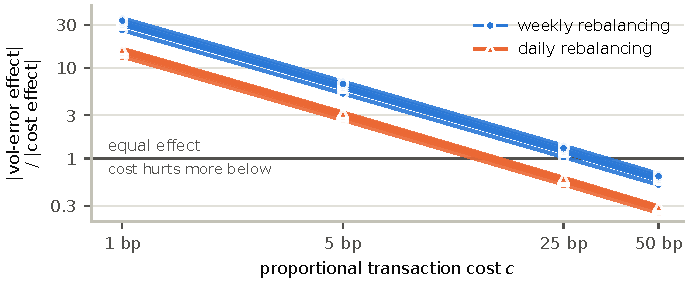
\includegraphics[width=0.76\linewidth]{fig_friction_ratio.pdf}
  \caption{Ratio of the \cvar{} effect of a $+10\%$ volatility error to that of proportional
    cost $c$, for the 12 contracts (lines join the four measured cost levels); above~1 the
    volatility error hurts more. Weekly and daily contracts form two bundles that cross~1 between
    25 and 50\bps{} and between 5 and 25\bps{}, respectively. Drawn by
    \texttt{paper/workshop/make\_figure.py} from \texttt{paper/findings\_sweep.json}.}
  \label{fig:friction}
\end{figure}

\paragraph{Mechanism: the ordering belongs to the tail.} On the \emph{mean}, closed forms hold in
all 12 contracts. With $\mu = r = 0$ the mean effect of the volatility error is exactly
$V(\sigma_h) - V(\sigma_r)$, matched to 0.3\%; the mean cost is Leland's rebalancing cost plus the
cost of opening and closing the hedge, matched to 3.5\% (Appendix~\ref{app:mechanism}). This is an
analytic check of the simulator and of the accounting, including the opening trade and the
terminal liquidation, which together carry 13--75\% of the cost. But \cvar{} is not a rescaled
mean. It amplifies the volatility
effect $1.6$--$3.0\times$ relative to its mean and the cost effect only $1.1$--$2.1\times$, so the
ordering in the tail differs from the ordering on the mean: at 25\bps{} the cost effect is the
larger in 10 of 12 contracts on the mean, but only in the 6 daily contracts on \cvar{}. Which
friction a benchmark finds first-order is a property of its risk measure as well as of the market.
A shortcut makes the point sharper. Leland's rebalancing-only ratio, $((1.1)^2 - 1)/\mathrm{Le}$
with $\mathrm{Le} = c\sqrt{8/\pi}/(\sigma\sqrt{\Delta t})$, tracks the \cvar{} ratios to within
28\% --- but only because the two things it omits, the opening and closing trades and the tail
amplification, roughly offset. An analytic prediction that agrees with a simulation can agree for
the wrong reason; decomposing the agreement is the check.

\paragraph{Calibration.} Both axes were set by assertion; we calibrate them from public data
(Appendix~\ref{app:calibration}). For the volatility error we compare realised S\&P~500
volatility over the 21 trading days after each close with VIX at that close, 1990--2026 (9{,}227
windows). The median ratio is $0.73$, and realised volatility is at least 10\% \emph{below} VIX in
78\% of windows, the favourable direction. It exceeds VIX by 10\% or more in 8.8\% of windows
(block-bootstrap 95\% CI 6.3--11.4\%) and by 25\% in 4.9\%: a $+10\%$ adverse error is about the
91st percentile, one month in eleven, and adverse months cluster at shock onsets. For costs, a
one-tick half-spread is 0.16\bps{} for E-mini S\&P~500 futures and 0.065\bps{} for SPY at current
index levels, and 1.6\bps{} for the median S\&P~500 constituent in 2015; 25--50\bps{} is small- and
micro-cap territory. VIX is not the volatility at which a desk hedges a given strike, and
one-year contracts are not calibrated here, so these are anchors rather than a joint model.

\paragraph{Implication.} For liquid underlyings, the adverse volatility error of a
one-month-in-eleven event costs more tail risk than any realistic proportional cost --- at the
E-mini's quoted spread the sweep's 5\bps{} corresponds to a quote 31 ticks wide --- so a protocol
that fixes volatility while sweeping costs varies the second-order axis. Costs dominate only for
illiquid underlyings under frequent rebalancing. Because adverse volatility errors concentrate in
market stress, when spreads tend to widen, the two axes are not independent either. A benchmark
should vary both, report
its conclusion under the risk measure it claims, and separate adverse from favourable errors.

% ======================================================================================
\section{Pitfall 4: too few seeds}\label{sec:noise}
% ======================================================================================

How many replicates a comparison needs depends on which source of variability dominates, and on
the power it demands.

\paragraph{Evaluation noise.} Over 100 independent replicates of the zero-cost delta hedge, the
SE of \cvar{} is $3.9$--$4.3\times$ that of the mean at equal path count ($0.0569$, $0.0268$ and
$0.0131$ at $N = 5{,}000$, $20{,}000$ and $100{,}000$ paths, against $0.0138$, $0.0069$ and
$0.0031$), so path counts must be set by the tail metric. Pairing strategies on common paths helps
the mean more than the tail. For band against delta at 50\bps{} (12 seeds of 20{,}000 paths),
pairing shrinks the s.d.\ of the difference $1.42\times$ for mean P\&L but only $1.19\times$ for
\cvar{} (paired s.d.\ $0.0480$), because the two strategies' tails are populated by different
paths. Only when one strategy is compared with itself under a perturbed parameter
(\S\ref{sec:friction}) does pairing make effects nearly deterministic. A ratio of s.d.s estimated
from few seeds is itself noisy: at 8 seeds of 10{,}000 paths the same two factors read $0.88$ and
$0.96$.

\paragraph{Training noise.} We trained 30 replicates of a feedforward policy (two hidden layers of
32 ReLU units; inputs $\tau/T$, $S/K$ and the previous position; unconstrained output) under the
entropic objective ($\lambda = 1$) at zero cost, for 2{,}000 Adam steps on fresh batches of 512
paths. Each replicate had its own initialisation and training paths, and all were scored on the
same 20{,}000 evaluation paths, isolating training variability. \cvar{} (loss orientation) had
mean $2.386$, range $[2.198, 2.665]$ and s.d.\ $s = 0.144$, 95\% CI $[0.115, 0.193]$: three times
the paired evaluation s.d.\ of the band-versus-delta comparison, so intervals from resampling test
paths alone would understate the uncertainty of a learned-policy comparison about threefold.

\begin{table}[t]
  \caption{Resolution and power implied by the training-seed noise floor at 2{,}000 steps
    ($s = 0.144$, 30 replicates) for an effect the size of band-versus-delta ($0.134$,
    Table~\ref{tab:band}).
    Power is for a two-sided $t$-test at $\alpha = 0.05$, from the noncentral $t$.}
  \label{tab:power}
  \centering
  \small
  % source: python -m experiments.findings noise_floor
  \begin{tabular}{rrrcc}
    \toprule
     & & 95\% CI & \multicolumn{2}{c}{Power} \\
    \cmidrule(lr){4-5}
    Seeds $k$ & $t_{0.975,\,k-1}$ & half-width & vs.\ fixed baseline & learned vs.\ learned \\
    \midrule
    5  & 2.776 & 0.179 & 0.36 & 0.26 \\
    6  & 2.571 & 0.151 & 0.46 & 0.31 \\
    10 & 2.262 & 0.103 & 0.75 & 0.51 \\
    12 & 2.201 & 0.091 & 0.84 & 0.59 \\
    20 & 2.093 & 0.067 & 0.98 & 0.82 \\
    \bottomrule
  \end{tabular}
\end{table}

\paragraph{Power.} Table~\ref{tab:power} gives, for $k$ seeds, the half-width of a 95\% CI and the
power to detect an effect the size of band-versus-delta, both against a fixed comparator
(one-sample $t$ on $k$ paired differences) and between two learned policies (two-sample $t$, $k$
per arm). Five seeds detect it with probability $0.36$. Power of 80\% needs 12 seeds against a
fixed comparator --- 8 to 19 across the CI of $s$ --- and 20 per arm between learned policies; for
half that effect, 39 and 74. A learned-versus-band difference may well be smaller than
band-versus-delta, so these counts are floors. \citet{colas2018seeds} make the same point for deep
reinforcement learning; what is new here are the domain quantities, for a tail-risk objective
whose training-seed noise exceeds its evaluation noise.

\paragraph{Longer training, and a run that failed.} At 8{,}000 steps the same 30 replicates improve
(mean \cvar{} $2.193$ against $2.386$) and their typical spread shrinks by more than half: the
robust s.d.\ (interquartile range$/1.349$) falls from $0.160$ to $0.063$. The s.d.\ barely moves,
$0.134$ (95\% CI $[0.107, 0.180]$), because one replicate did not converge. Its training loss fell
to about $0.65$ by step 3{,}000, like the others, then rose to $1.4$ by step 4{,}500 and settled near
$1.0$, while a typical run went on to $0.58$; its \cvar{} ended at $2.833$, 11 robust s.d.s from
the median, having been unremarkable at 2{,}000 steps ($2.483$, ninth worst of 30). Without it the
s.d.\ is $0.059$. A replicate's score at 2{,}000 steps barely predicts its score at 8{,}000
(correlation $0.17$), so early ranking would not have caught it. Nor did the convergence check this
project first used --- last-decile loss below first-decile loss, which the initialisation spike
satisfies --- whereas the ratio of final-window to best-window loss flags it ($+55\%$, against
about zero for converged runs). One failure in 30 is a rate with a wide interval
(Clopper--Pearson 95\%: 0.1--17\%), but at the observed rate a 12-seed study contains a failed run
with probability $0.33$, and a comparison with 20 runs per arm with probability $0.74$. A power
calculation on the s.d.\ treats such a run as Gaussian noise, and it is not. Seed counts must be set
at the training budget actually used, and failed runs counted by a criterion fixed before seeing
outcomes, reported, and never dropped, with robust aggregates such as the interquartile mean
\citep{agarwal2021deep} alongside the mean.

\paragraph{Two corrections we record.} An earlier version of our analysis computed the seed
requirement with a normal critical value of $2.0$ and concluded that four seeds sufficed;
$t_{0.975,4} = 2.776$ is 39\% larger. A later version reported the 95\% CI half-width as a
``minimum detectable effect'' and concluded that six seeds sufficed, but an effect equal to that
half-width is detected only about half the time; and its $s$ came from 8 replicates ($0.122$),
whose own CI spanned 6 to 29 seeds. Tests now pin the $t$ critical value, the power calculation
(checked against 200{,}000 simulated $t$-tests per seed count), and the gap between a CI
half-width and an 80\%-power effect.

% ======================================================================================
\section{Pitfall 5: an underspecified acceptance gate}\label{sec:gate}
% ======================================================================================

A verification ladder is only as good as its gates. Ours required, before any learned-policy
result could be reported, that a policy trained at zero cost recover the Black--Scholes delta:
mean absolute deviation (MAD) below $0.05$ and maximum deviation below $0.15$ against
$\Phi(d_1)$ over the region $R = \{S/K \in [0.8, 1.2],\ \tau \in [0.1, 1]\}$. The gate was
written before any policy was trained, and it looked complete. It is not. It leaves two choices
unstated: (i) the value of the previous-position input when the policy is evaluated on a grid of
$(\tau, S)$ --- the optimal zero-cost hedge ignores that input, but the network receives it --- and
(ii) how the states in $R$ are weighted, uniformly on a grid or as the policy visits them.

Table~\ref{tab:gate} scores six replicates (8{,}000 Adam steps each, otherwise as in
\S\ref{sec:noise}) under three designs over the same region: a grid with the previous position
set to 0; a grid with it set to $\Phi(d_1)$, close to the position a well-trained policy holds
along its own paths; and the states visited by the policy's own rollouts on 20{,}000 evaluation
paths. Our log recorded the gate
as failed on the first trained policy (MAD $0.074$ under the first design). The same network
passes under either other design, as do all six replicates; under the first design one of six
passes.

\begin{table}[t]
  \caption{One gate, three evaluation designs: deviation from $\Phi(d_1)$ over $R$, mean $\pm$
    s.d.\ across 6 training replicates. Gate: MAD $< 0.05$ and max $< 0.15$.}
  \label{tab:gate}
  \centering
  \small
  % source: python -m experiments.findings evaluation_design
  \begin{tabular}{lccc}
    \toprule
    Evaluation design & MAD & Max deviation & Replicates passing \\
    \midrule
    Grid, previous position $= 0$           & $0.053 \pm 0.014$ & $0.173 \pm 0.038$ & 1/6 \\
    Grid, previous position $= \Phi(d_1)$   & $0.034 \pm 0.007$ & $0.097 \pm 0.011$ & 6/6 \\
    States visited by the policy            & $0.027 \pm 0.005$ & $0.119 \pm 0.017$ & 6/6 \\
    \bottomrule
  \end{tabular}
\end{table}

\paragraph{The check the gate lacked.} The disagreement has a cause that the gate could have
tested directly. At zero cost the optimal policy is Markov in $(t, S)$, so its output cannot depend
on the previous position. Moving only that input from 0 to 1 at each grid point moves the trained
networks' outputs by $0.052 \pm 0.019$ on average, and by up to $0.21$: the networks use an input
the target ignores. This shortcut is nearly invisible on the states the policy visits, where the
previous position is close to $\Phi(d_1)$, and exposed off them; a grid with the previous position
at 0 is realistic only at $t_0$. A well-posed gate states its conditioning and its weighting,
reports both, and includes an invariance check on every input the target is known not to depend
on. We claim this rung in neither direction; it will be re-run under a gate re-specified in this
way.

% ======================================================================================
\section{Recommendations: executable checks}\label{sec:recs}
% ======================================================================================

Each recommendation is an executable check or a reporting rule. The checks are implemented in the
repository and pinned by tests, except the re-specified gate of item~5, whose test is written but
not yet run.
\begin{enumerate}
\item \textbf{Replicate streams.} Derive seeds by hashing (stream label, index), pass list seeds, or
  split one generator; never pass replicate indices as integers to \fromseed{}. Check the
  cross-replicate dispersion of an estimator against its analytic SE; lag-0 correlations and
  same-seed reruns cannot see shifted streams.
\item \textbf{The classical baseline.} Implement the band as a clip to its edges, so that trade-to-centre
  is unrepresentable, and check that it beats delta hedging on both \cvar{} and turnover.
\item \textbf{Frictions.} Vary volatility error, adverse and favourable separately, as well as cost,
  each calibrated to the instrument. Check simulated mean effects against closed forms, and report
  which friction dominates under the risk measure the claim uses.
\item \textbf{Replicates.} Size path counts by the tail metric, and seed counts by power from a
  noise floor measured at the training budget used, carrying the uncertainty of its s.d. Flag
  failed runs from their loss histories by a criterion fixed in advance; report them and never
  drop them. Report comparisons below 80\% power as inconclusive rather than null.
\item \textbf{Acceptance gates.} State the conditioning of every input and the weighting over states,
  report both natural designs, and test invariance to inputs the target ignores.
\item \textbf{Provenance.} Regenerate every number from committed code and pin each claim with a
  test, including negative tests that keep withdrawn claims from returning.
\end{enumerate}

% ======================================================================================
\section{Related work}\label{sec:related}
% ======================================================================================

\paragraph{Deep hedging and its evaluation.} Deep hedging optimises a convex risk measure of
simulated P\&L directly \citep{buehler2019deep}. Recent work studies robustness to distributional
shift through adversarial training \citep{he2025distributional}, training across
parameter-uncertainty sets \citep{lutkebohmert2022robust}, architectures with a built-in
no-transaction band \citep{imaki2023ntb}, valuation adjustments for execution under frictions
\citep{sakuma2026robust}, and comparison against cost-aware classical rules on market data
\citep{kumar2026deep}. Reviews note that neural-hedging conclusions depend on the benchmark chosen
and on leakage-free data splits \citep{ruf2020neural}, and that the field lacks a standard
benchmark \citep{pickard2023deep}. Our measurements concern the evaluation apparatus rather than
any hedging method; they are complementary to these studies, and we make no claim about their
results.

\paragraph{Evaluation statistics.} Seed variability alone can produce statistically different
results from identical configurations \citep{henderson2018deep}; power analysis should set seed
counts \citep{colas2018seeds}; interval estimates should replace point estimates when runs are few
\citep{agarwal2021deep}; and correlated replicates inflate the variance of benchmark estimates
\citep{bouthillier2021accounting}. Inference from non-independent replicates is a classical error
of experimental design \citep{hurlbert1984pseudoreplication}. We measure these quantities for a
tail-risk objective in hedging, and show a route by which replicates become non-independent with
no deliberate choice at all.

\paragraph{Random streams.} Counter-based generators give independent streams through distinct keys
or disjoint counter ranges \citep{salmon2011parallel}; related seeds producing correlated streams
is a known defect class \citep{matsumoto2007common}; and TensorFlow's guide warns about overlapping
streams from \fromseed{} \citep{tensorflow2024guide}. We document the deterministic integer path
behind that warning, and its statistical consequence.

\paragraph{Evaluation pitfalls in financial machine learning.} At NeurIPS, evaluation validity in
finance has centred on look-ahead leakage in backtests of language-model agents
\citep{li2025deepfund}. Ours is the complementary, simulation-side question: when replicates,
ground truth and closed forms are all available, what still goes wrong?

% ======================================================================================
\section{Limitations}\label{sec:limits}
% ======================================================================================

\begin{itemize}
\item \textbf{One world, one claim type.} European calls under geometric Brownian motion, with no
  stochastic volatility or jumps; the sweep covers 12 contracts, the other findings one ATM
  contract. Market data enter only to calibrate the two friction axes, for the S\&P~500 index;
  VIX is not the implied volatility of a specific strike, and one-year horizons are not calibrated.
\item \textbf{A framework-specific mechanism.} Pitfall~1 concerns \fromseed{} with TensorFlow~2.21's
  Philox generator. We have not examined other versions or frameworks; tests pin the mechanism so
  that a change fails loudly.
\item \textbf{One noise-floor configuration.} One architecture and one objective (entropic, zero
  cost) at two budgets, with a constant learning rate; one failure in 30 runs estimates the
  failure rate only loosely. The noise floor of a cost-aware policy may differ, and seed counts
  should be re-derived for each comparison from its own measured floor.
\item \textbf{No learned-policy accuracy is claimed.} The rung-4 gate is being re-specified
  (\S\ref{sec:gate}).
\item \textbf{No learned-versus-classical comparison is claimed:} the paper concerns the
  measurement apparatus, not whether deep hedging beats, ties or loses to the band.
\item \textbf{Reproducibility gaps.} Findings are parameterised in code
  (\texttt{experiments/findings.py}) rather than by the YAML configurations the project
  specifies, whose runner is not yet implemented. Market data cannot be redistributed, so the
  calibration regenerates only after a download; its arithmetic is unit-tested on synthetic data.
\item \textbf{Literature coverage.} Claims about other work are restricted to sources read in
  full; we make no claim about the practices of published work in general.
\end{itemize}

% ======================================================================================
\begin{ack}
\textbf{[AUTHOR --- approve or edit this disclosure.]} Substantial portions of the code, the
analysis and the text were produced with the assistance of an AI coding assistant (Claude,
Anthropic), under the author's direction. All reported numbers are regenerated by committed code;
all except the market calibration are pinned by automated tests; and every claim about other work
is recorded, with page references to the source text, in \texttt{docs/07-literature-audit.md}.
\textbf{[AUTHOR --- funding and competing-interests statement.]}
\end{ack}

{\small
\bibliographystyle{plainnat}
\bibliography{references}
}

% ======================================================================================
\appendix
% ======================================================================================

\section{Reproducibility}\label{app:repro}

\paragraph{Environment.} TensorFlow~2.21, Keras~3.15, NumPy~2.2.6, SciPy, Python~3.12, on a laptop
CPU; no GPU was used. Code: \url{https://github.com/Adi7710/deep-hedging-benchmark}.
\textbf{[AUTHOR --- record the commit hash and the test-suite result at submission.]}

\paragraph{Commands and tests.} Commands run from the repository root; adding
\texttt{-{}-all -{}-json <path>} to \texttt{python -m experiments.findings} runs every finding
and writes a machine-readable record. Tests (under \texttt{tests/}) pin each claim's direction,
ordering and significance at reduced sample sizes, not its exact value.

{\raggedright
\begin{description}\small
\item[Tables~\ref{tab:mechanism} and~\ref{tab:consequence} (seeding).] Command:
  \texttt{python -m experiments.findings seeding}. Tests (\texttt{test\_seeding.py}):
  \path{test_integer_seed_is_written_into_the_philox_counter},
  \path{test_consecutive_integer_seeds_are_shifted_copies},
  \path{test_lag_zero_correlation_cannot_see_the_overlap},
  \path{test_a_list_seed_lands_in_the_key},
  \path{test_hashed_replicates_are_not_shifted_copies},
  \path{test_cross_seed_dispersion_matches_analytic_standard_error}.
\item[Table~\ref{tab:band} (band rebalancing).] Command:
  \texttt{python -m experiments.findings baseline}. Tests (\texttt{test\_findings.py}):
  \path{test_band_edge_beats_band_centre_beats_delta},
  \path{test_the_edge_rule_advantage_is_significant_and_consistent},
  \path{test_the_centre_over_edge_ratio_is_not_estimable}; and
  (\texttt{test\_rungs\_3\_to\_6.py}) \path{test_band_hedging_beats_naive_delta_under_costs}.
\item[Table~\ref{tab:sweep}, Figure~\ref{fig:friction}, Tables~\ref{tab:sweep-vol}--\ref{tab:sweep-cost} (friction sweep).]
  Command: \texttt{python -m experiments.findings misspecification\_sweep}, stored in
  \texttt{paper/findings\_sweep.json}; figure by \texttt{python paper/workshop/make\_figure.py}.
  Tests: \path{test_adverse_vol_error_dominates_index_like_costs_in_every_contract},
  \path{test_favourable_vol_error_is_a_gain},
  \path{test_the_ordering_flips_at_illiquid_underlying_costs},
  \path{test_daily_rebalancing_narrows_the_ratio}.
\item[Table~\ref{tab:mechanism-full} (friction mechanism).] Command:
  \texttt{python -m experiments.findings friction\_mechanism}. Tests:
  \path{test_mean_effects_match_closed_forms},
  \path{test_the_tail_metric_amplifies_vol_error_more_than_cost},
  \path{test_which_friction_dominates_depends_on_the_risk_measure}.
\item[Table~\ref{tab:calibration} (market calibration).] Command:
  \texttt{python -m experiments.market\_calibration -{}-cache-dir <outside the repo>
  -{}-json paper/market\_calibration.json} (downloads public data; raw files never enter the
  repository). Tests (\texttt{test\_market\_calibration.py}) pin the realised-volatility windows,
  the cost conversion, bootstrap determinism, and the refusal to cache raw data in a tracked path.
\item[Section~\ref{sec:noise} (evaluation noise).] Commands:
  \texttt{python -m experiments.findings precision\_by\_n} (100 replicates) and
  \texttt{python -m experiments.findings precision} (paired s.d.\ and pairing factors). Tests:
  \path{test_tail_metric_se_exceeds_the_mean_se_several_fold},
  \path{test_cvar_is_substantially_noisier_than_the_mean},
  \path{test_common_random_numbers_help_but_only_modestly}.
\item[Table~\ref{tab:power} and the 8{,}000-step result (noise floor and power).] Commands:
  \texttt{python -m experiments.findings noise\_floor} (30 replicates, 2{,}000 steps) and
  \texttt{noise\_floor\_long} (8{,}000 steps; both report each run's loss-history diagnostics
  and the robust spread). Tests:
  \path{test_ci_halfwidth_uses_the_t_critical_value},
  \path{test_the_ci_halfwidth_is_not_an_80pct_power_mde},
  \path{test_power_reproduces_an_independent_calculation},
  \path{test_learned_vs_learned_needs_more_seeds_than_vs_a_fixed_comparator},
  \path{test_the_loss_history_check_catches_a_run_that_regressed},
  \path{test_robust_z_flags_a_planted_failed_run}.
\item[Table~\ref{tab:gate} (acceptance gate).] Command:
  \texttt{python -m experiments.findings evaluation\_design}.
\item[Section~\ref{sec:setup} checks.] \path{test_mc_price_matches_black_scholes}
  (\texttt{test\_rung1\_mc\_price.py}); \texttt{python -m experiments.findings convergence} and
  \path{test_delta_hedge_error_shrinks_with_rebalancing} (\texttt{test\_rung2\_pnl\_accounting.py});
  \path{test_transaction_costs_includes_final_liquidation};
  \path{test_empirical_cvar_matches_the_training_objective_at_its_optimum}
  (\texttt{test\_metrics.py}); \path{test_band_width_scales_as_cube_root_of_cost}.
\end{description}
}

\paragraph{Compute.} Every experiment ran on a laptop CPU. Compiling the training step with
\texttt{tf.function} cut the time per gradient step from 92.4\,ms to 5.5\,ms ($16.9\times$), so a
2{,}000-step training run takes about 11\,s; compiled and eager training give the same loss
history to within $10^{-4}$ (\path{test_compiled_and_eager_training_agree}). The largest findings
(the 30-replicate noise floor, the friction sweep) take minutes to tens of minutes each.

\section{Full friction sweep}\label{app:sweep}

Tables~\ref{tab:sweep-vol} and~\ref{tab:sweep-cost} give every effect of \S\ref{sec:friction}
as mean (s.d.\ across 3 seeds, in units of $10^{-3}$). Each effect is a paired difference in
\cvar{} (P\&L orientation) against the correctly specified zero-cost delta hedge of the same
contract; 40{,}000 paths per seed.

\begin{table}[h]
  \caption{Volatility-error effects: realised $\sigma_r = \rho\,\sigma_h$, $\sigma_h = 0.2$,
    zero cost. Mean (s.d.\ $\times 10^{3}$).}
  \label{tab:sweep-vol}
  \centering
  \footnotesize
  % source: python -m experiments.findings misspecification_sweep -> paper/findings_sweep.json
  \begin{tabular}{rrcr rrrr}
    \toprule
    $K$ & $T$ & & $n$ & $\rho = 0.8$ & $\rho = 0.9$ & $\rho = 1.1$ & $\rho = 1.25$ \\
    \midrule
    90 & 0.25 & W & 13 & $+1.159$\,(12.03) & $+0.634$\,(3.54) & $-0.687$\,(3.99) & $-1.792$\,(11.65) \\
    90 & 1 & W & 52 & $+1.871$\,(7.64) & $+1.086$\,(5.54) & $-1.232$\,(9.67) & $-3.241$\,(24.40) \\
    100 & 0.25 & W & 13 & $+1.410$\,(8.06) & $+0.743$\,(3.08) & $-0.799$\,(2.60) & $-2.073$\,(6.41) \\
    100 & 1 & W & 52 & $+2.175$\,(19.45) & $+1.222$\,(9.82) & $-1.370$\,(7.70) & $-3.598$\,(13.24) \\
    110 & 0.25 & W & 13 & $+1.415$\,(4.90) & $+0.768$\,(0.51) & $-0.829$\,(5.64) & $-2.164$\,(16.50) \\
    110 & 1 & W & 52 & $+2.208$\,(14.71) & $+1.296$\,(7.42) & $-1.471$\,(7.38) & $-3.872$\,(10.86) \\
    \midrule
    90 & 0.25 & D & 63 & $+0.714$\,(7.09) & $+0.466$\,(3.89) & $-0.559$\,(6.77) & $-1.496$\,(11.38) \\
    90 & 1 & D & 252 & $+1.183$\,(14.19) & $+0.849$\,(11.79) & $-1.136$\,(4.89) & $-3.032$\,(20.67) \\
    100 & 0.25 & D & 63 & $+1.048$\,(5.61) & $+0.601$\,(5.14) & $-0.681$\,(4.72) & $-1.790$\,(8.41) \\
    100 & 1 & D & 252 & $+1.493$\,(13.68) & $+0.984$\,(10.31) & $-1.276$\,(6.53) & $-3.397$\,(18.95) \\
    110 & 0.25 & D & 63 & $+0.879$\,(6.93) & $+0.572$\,(5.76) & $-0.681$\,(12.95) & $-1.818$\,(21.17) \\
    110 & 1 & D & 252 & $+1.336$\,(0.84) & $+0.989$\,(0.93) & $-1.359$\,(5.93) & $-3.637$\,(8.02) \\
    \bottomrule
  \end{tabular}
\end{table}

\begin{table}[h]
  \caption{Cost effects: proportional cost $c$, $\sigma_r = \sigma_h = 0.2$. Mean (s.d.\
    $\times 10^{3}$).}
  \label{tab:sweep-cost}
  \centering
  \footnotesize
  % source: python -m experiments.findings misspecification_sweep -> paper/findings_sweep.json
  \begin{tabular}{rrcr rrrr}
    \toprule
    $K$ & $T$ & & $n$ & 1\bps{} & 5\bps{} & 25\bps{} & 50\bps{} \\
    \midrule
    90 & 0.25 & W & 13 & $-0.026$\,(0.11) & $-0.131$\,(0.50) & $-0.664$\,(1.87) & $-1.347$\,(3.65) \\
    90 & 1 & W & 52 & $-0.041$\,(0.08) & $-0.206$\,(0.30) & $-1.052$\,(1.20) & $-2.142$\,(4.58) \\
    100 & 0.25 & W & 13 & $-0.027$\,(0.18) & $-0.133$\,(0.97) & $-0.679$\,(3.76) & $-1.386$\,(6.58) \\
    100 & 1 & W & 52 & $-0.043$\,(0.34) & $-0.218$\,(1.69) & $-1.114$\,(5.71) & $-2.274$\,(9.28) \\
    110 & 0.25 & W & 13 & $-0.023$\,(0.14) & $-0.117$\,(0.69) & $-0.598$\,(3.88) & $-1.227$\,(8.08) \\
    110 & 1 & W & 52 & $-0.044$\,(0.23) & $-0.221$\,(1.08) & $-1.134$\,(5.60) & $-2.320$\,(11.16) \\
    \midrule
    90 & 0.25 & D & 63 & $-0.042$\,(0.24) & $-0.210$\,(0.97) & $-1.087$\,(2.90) & $-2.234$\,(3.63) \\
    90 & 1 & D & 252 & $-0.075$\,(0.36) & $-0.382$\,(2.00) & $-2.003$\,(8.72) & $-4.121$\,(12.40) \\
    100 & 0.25 & D & 63 & $-0.046$\,(0.18) & $-0.235$\,(0.59) & $-1.218$\,(3.24) & $-2.503$\,(5.85) \\
    100 & 1 & D & 252 & $-0.082$\,(0.43) & $-0.416$\,(1.61) & $-2.185$\,(6.00) & $-4.498$\,(14.06) \\
    110 & 0.25 & D & 63 & $-0.041$\,(0.11) & $-0.210$\,(0.59) & $-1.110$\,(1.54) & $-2.302$\,(1.59) \\
    110 & 1 & D & 252 & $-0.084$\,(0.25) & $-0.429$\,(1.45) & $-2.265$\,(4.33) & $-4.676$\,(7.16) \\
    \bottomrule
  \end{tabular}
\end{table}

\section{The friction ordering, decomposed}\label{app:mechanism}

Leland's adjustment prices a one-way proportional cost $c$, paid at rebalances $\Delta t$ apart,
as extra variance $\sigma^2(1 + \mathrm{Le})$, $\mathrm{Le} = c\sqrt{8/\pi}/(\sigma\sqrt{\Delta
t})$ \citep{leland1985option}. With $\mu = r = 0$ and
$G = \mathbb{E}\big[\tfrac12\int_0^T \Gamma S^2 \sigma^2\, dt\big] = \sigma\,\mathrm{Vega}/2$, the
mean effects have closed forms: the volatility error costs exactly $V(\sigma_h) - V(\sigma_r)$, and
the cost is, to first order, $\mathrm{Le}\,G + c\,S_0\,(\Delta_0 + \Phi(d_1))$ --- rebalancing plus
opening and closing the hedge, since $\mathbb{E}[S_n \delta_{n-1}] \approx S_0 \Phi(d_1)$ when
$\mu = 0$. Table~\ref{tab:mechanism-full} compares both with simulation, on the draws of
Table~\ref{tab:sweep}, and sets the mean ratios beside the \cvar{} ratios.

\begin{table}[h]
  \caption{Mean versus \cvar{} effects, 3 seeds of 40{,}000 paths. Vol: effect of $\rho = 1.1$.
    5\bps{}: effect of cost. Sim/exact and sim/pred: simulated mean against the closed form.
    Rebal.: share of the 5\bps{} cost spent on rebalancing (the rest opens and closes the hedge).
    Amp.: \cvar{} effect over mean effect. Ratios: $|$vol$|$ over $|$cost$|$ at 5 and 25\bps{}.}
  \label{tab:mechanism-full}
  \centering
  \scriptsize
  \setlength{\tabcolsep}{2.6pt}
  % source: python -m experiments.findings friction_mechanism
  \begin{tabular}{rrcr rr rr r rr rr rr}
    \toprule
     & & & & \multicolumn{2}{c}{Vol mean} & \multicolumn{2}{c}{5\bps{} mean} & & \multicolumn{2}{c}{Amp.} & \multicolumn{2}{c}{Ratio, 5\bps{}} & \multicolumn{2}{c}{Ratio, 25\bps{}} \\
    \cmidrule(lr){5-6}\cmidrule(lr){7-8}\cmidrule(lr){10-11}\cmidrule(lr){12-13}\cmidrule(lr){14-15}
    $K$ & $T$ & & $n$ & sim & exact & sim & pred & Rebal. & vol & 5\bps{} & mean & \cvar{} & mean & \cvar{} \\
    \midrule
    90 & 0.25 & W & 13 & $-0.228$ & $-0.228$ & $-0.1161$ & $-0.1177$ & 25\% & 3.01 & 1.13 & 1.97 & 5.24 & 0.39 & 1.03 \\
    90 & 1 & W & 52 & $-0.663$ & $-0.664$ & $-0.1667$ & $-0.1678$ & 56\% & 1.86 & 1.24 & 3.98 & 5.97 & 0.80 & 1.17 \\
    100 & 0.25 & W & 13 & $-0.399$ & $-0.398$ & $-0.1066$ & $-0.1093$ & 51\% & 2.00 & 1.25 & 3.74 & 6.00 & 0.75 & 1.18 \\
    100 & 1 & W & 52 & $-0.792$ & $-0.793$ & $-0.1669$ & $-0.1682$ & 68\% & 1.73 & 1.31 & 4.74 & 6.29 & 0.95 & 1.23 \\
    110 & 0.25 & W & 13 & $-0.277$ & $-0.277$ & $-0.0545$ & $-0.0565$ & 66\% & 2.99 & 2.14 & 5.08 & 7.11 & 1.02 & 1.39 \\
    110 & 1 & W & 52 & $-0.751$ & $-0.751$ & $-0.1413$ & $-0.1422$ & 75\% & 1.96 & 1.56 & 5.31 & 6.65 & 1.06 & 1.30 \\
    \midrule
    90 & 0.25 & D & 63 & $-0.228$ & $-0.228$ & $-0.1546$ & $-0.1552$ & 44\% & 2.45 & 1.36 & 1.48 & 2.66 & 0.30 & 0.51 \\
    90 & 1 & D & 252 & $-0.663$ & $-0.664$ & $-0.2806$ & $-0.2811$ & 74\% & 1.71 & 1.36 & 2.36 & 2.98 & 0.47 & 0.57 \\
    100 & 0.25 & D & 63 & $-0.397$ & $-0.398$ & $-0.1770$ & $-0.1782$ & 71\% & 1.71 & 1.33 & 2.25 & 2.90 & 0.45 & 0.56 \\
    100 & 1 & D & 252 & $-0.792$ & $-0.793$ & $-0.3047$ & $-0.3054$ & 82\% & 1.61 & 1.37 & 2.60 & 3.07 & 0.52 & 0.58 \\
    110 & 0.25 & D & 63 & $-0.277$ & $-0.277$ & $-0.1018$ & $-0.1023$ & 82\% & 2.46 & 2.07 & 2.72 & 3.23 & 0.54 & 0.61 \\
    110 & 1 & D & 252 & $-0.751$ & $-0.751$ & $-0.2704$ & $-0.2707$ & 87\% & 1.81 & 1.59 & 2.78 & 3.17 & 0.56 & 0.60 \\
    \bottomrule
  \end{tabular}
\end{table}

\section{Market calibration}\label{app:calibration}

Realised volatility is $\mathrm{RV}_t = \sqrt{(252/21)\sum_{k=1}^{21} r_{t+k}^2}$ from S\&P~500
closes (not demeaned), set against VIX at the close of day $t$; the ratio is exactly the sweep's
$\rho$ when the hedge runs at implied volatility. Overlapping windows are handled by a circular
block bootstrap (252-day blocks; 63 and 504 give the same interval to 0.5 percentage points) and
by the 21 non-overlapping subsamples. A proportional one-way cost for an instrument quoted one
tick wide is $c = (\text{tick}/2)/\text{price}$. Sources and licensing are recorded in
\texttt{experiments/market\_calibration.py}; the headline was recomputed independently from
Cboe's own VIX and SPX files.

\begin{table}[h]
  \caption{Calibration of the two friction axes (strike dates 1990-01-02 to 2026-08-26).}
  \label{tab:calibration}
  \centering
  \small
  % source: python -m experiments.market_calibration -> paper/market_calibration.json
  \begin{tabular}{lr}
    \toprule
    Quantity & Value \\
    \midrule
    Windows (overlapping; approx.\ independent) & 9{,}227; 440 \\
    Median $\mathrm{RV}/\mathrm{VIX}$ & 0.73 \\
    $\Pr(\mathrm{RV} < 0.9\,\mathrm{VIX})$, favourable & 78.1\% \\
    $\Pr(\mathrm{RV} > 1.1\,\mathrm{VIX})$ [95\% block-bootstrap CI] & 8.8\% [6.3, 11.4] \\
    $\Pr(\mathrm{RV} > 1.1\,\mathrm{VIX})$, range over non-overlapping offsets & 7.5--10.0\% \\
    $\Pr(\mathrm{RV} > 1.25\,\mathrm{VIX})$ & 4.9\% \\
    One-tick half-spread, E-mini S\&P~500 (2026-09-25; 1998--2026 range) & 0.16\bps{} (0.16--1.85) \\
    One-cent half-spread, SPY (2026-09-25) & 0.065\bps{} \\
    Quoted half-spread, median S\&P~500 constituent (Dec.\ 2015) & 1.6\bps{} \\
    Quoted half-spread, \$100M--\$1bn stocks (2013 medians) & 7.8--61\bps{} \\
    \bottomrule
  \end{tabular}
\end{table}

\end{document}
